% !Mode:: "TeX:UTF-8"
\chapter{绪论}

\section{研究的背景与意义}

面对人们日益加剧的信息分享和获取的需求,硬件方面智能终端设备也在不
断的推陈出新,而同样的,在软件方面,移动互联网也逐渐渗透到各行各业当中, 
产生了几个概念,比如“互联网+”和“工业 4.0”。
全世界进入了一个新的时代,一个属于移动互联网的新时代。
编程语言虽然是链接计算机硬件与软件的桥梁,但是由于编程语言并不直接面向用户,
各种各样的编程语言,只能说是整个信息技术的发展与繁荣的幕后功臣。
编程语言 ( programming language ) 的发展,和计算机技术的发展几乎同步,从机器语言 ( machine language ) 到汇编语言 ( assembly language ),再发展到高级语言 ( high-level language )。
从结构化编程语言 ( Structured programming language ),发展到面向对象的编程语言 ( Object oriented programming language )。编程语言的演进过程,也是人们 (业界) 对于编程语言的需求不断变化的结果。

然而,新的编程语言的出现,往往会伴随着就有编程语言的衰落,
而导致大量基于旧的编程语言编写的系统变为遗留系统。
这些遗留系统和传统软件在更新或者重用过程中,可能需要对海量代码进行重构和移植,
需要消耗极其大量的人力和物力。
如何简单有效的进行软件的移植工作,是业界一直存在的一个普遍问题。

HTML5于2004年正式被提出。过了十年之久,直到微信出现才正式被关注。
并随着微信的升温,HTML5也随之火了起来。
HTML5是web开发世界的一次重大的改变,随着智能手机的发展, 
Apple的支持, Adobe围绕HTML5的产品开发,以及移动flash的死亡等,
Html5毅然成为了发展方向。它代表着未来趋势。

HTML5有相比传统的web有以下几个显著优势:

\begin{itemize}
    \item {\heiti 移动网站:}H5主要针对移动网站,今日的成就绝对归功与智能手机
    \item {\heiti 代码简洁:}H5代码更加简洁,修改更灵活
    \item {\heiti 浏览器兼容:}Chrome、Firefox、Safari、IE9 和 Opera都支持 
    \item {\heiti 交互性:}通过 HTML5 的绘图标签 ( canvas标签 ),配合JavaScript代码,可以实现大多数的交互操作和动态效果,而不需要flash
    \item {\heiti 本地存储:}H5有点像传统的cookie技术和客户端数据库的跨界组合。
    \item {\heiti 视频音频:}可以不使用Flash 播放器和其它的第三方媒体播放器,HTML5已经支持了音频视频功能
    \item {\heiti W3C标准:}H5满足网页w3c标准
\end{itemize}


从上个世纪 90 年代开始,随着个人机的兴起,以及计算机价格的不断下降,客户机/服务器架构(Client/Server architecture,以下简称为 C/S 架构)逐渐取代了
曾经红极一时的主机/终端机架构(Host/Terminal architecture),产生了巨大的社会价值,极大推动了IT行业的发展。
但随着移动互联网 (mobile web) 的不断普及以及移动设备应用 (mobile app) 的迅速迭代敏捷开发快速升级的要求,传统 C/S 架构的应用已经感到有些力不从心。
而 Web 平台是一个和传统桌面平台完全不同的平台,web平台的特点是调度任务集中,云端化,并且以用户体验为中心;
它是一个分布式、面向所有用户、高可用、高性能 (性能足够高) 、端到端的平台;
它能使企业在推广业务时获取更多竞争优势。
但是,很多企业可能并没有那么多人力物力来重新进行 web 版的编写,
如果能有一种技术,既能使用传统软件的源代码,直接生成 web 版的应用,或者能生 
成关键模块,简化 web 应用的开发过程,对于企业的发展极为有用。

\section{本课题研究现状}

\subsection{软件移植理论相关进展}

软件移植\upcite{krueger1992software}
指经过对原有软件的修改,是其运行在一个新的环境的过程,
该过程在软件工程理论中的软件生命周期中属于软件的维护阶段。
黄聪惠等学者\upcite{黄聪会2012软件移植理论与技术研究}指出软件移植
是一个使遗留系统适应新的软硬件环境的移动过程,要求软件移植时至少要保证软件的基本功能,
从而延长软件自身的生命周期。不过,本人认为,软件移植减少新平台开发的成本才是最重要的作用。

软件移植的研究主要分两个部分:研究软件的可移植性理论和
研究具体软件移植的实现方法或探究通用的移植方法。将C++语言移植到html5平台/JavaScript语言属于
研究针对某个具体问题的的软件移植实现方法。

软件移植是软件重用的一种重要形式。通过软件移植与软件重用的比较,可以更深入的理解软件移植的概念。
魏仁选等专家\upcite{魏仁选2002软件重用与移植的比较研究}总结了软件移植与软件重用的区别。
他们认为:软件移植研究的目的在于促进原有软件系统在新环境的重用,
而软件重用是实现一个软件系统的软件制品在多种情形下 (比如不同的操作系统,不同的体系结构,不同的硬件配置等) 的、广泛的重复使用。
二者的区别在于软件移植实现旧有软件在新平台和新环境下的运行,
而软件重用则着重于构建和维护软件构件集以便于实现在新软件在多种环境中的重复利用。
简单来说,软件重用在开发时就已经开始考虑移植性、跨平台等问题,而软件移植是已有软件基础上的二次开发工作。拿android和ios举例子,把一个android app迁移到ios平台是软件移植;而先开发一个android和ios通用开发框架,然后在此框架的基础上开发跨平台app则属于软件重用。
软件移植在研究的目的和所涉及的范围上已经软件开发周期中所属的时间都和软件重用不同。

软件的移植在不同的时期表现出了不同的特点\upcite{王建房2011从}。
早期的软件移植的主要问题很简单。就是解决旧有软件移植到和旧有软件别的体系结构或者另外的操作系统或者体系结构和操作系统两者都不相同,
以应对当时市场上的硬件和操作系统多样化、复杂化的特点,
基于图标、窗口、按钮和鼠标的图形用户界面问世后,软件移植转向CLI向GUI迁移。
Smalltalk、Visual C++、Delphi等IDE的出现极大的改善开发者们的开发环境,简化了开发者的开发方式,
这时软件移植的重点也变为了在保留命令行程序结构化逻辑的前提下,在图形界面下的再实现,举个简单的例子,点击菜单栏里的某个按钮,执行某个功能,这些功能往往是命令行时代本来就有的。

软件移植工作主要分为\upcite{krueger1992software}软件源代码移植与二进制文件移植两种。
源代码移植:通过修改与环境相关的部分源代码 (尽可能不修改主要逻辑,主要是解决环境依赖相关的问题) ,使软件具备适应另外的软件硬件环境的能力;
而二进制移植是指直接在目的环境下执行原有软件,通过填补目标环境与原有环境的不同 (类库接口映射,虚拟机等形式),使目标软件可以在目标平台下运行,并与其在源环境下行为保持一致。最著名的例子,就是wine项目\upcite{amstadt1994wine},可以直接在linux下运行windows平台的应用,把directx和MFC直接映射到openGL和X11时其实现的巧妙令人惊艳。

源代码移植方法的研究主要分为源代码移植的一般方法 (通用方法) 的研究和针对具体软件的移植的方法研究。对源代码移植的一般方法研究对软件移植工作的展开有这重要的指导意义。Fleuery\upcite{fleurey2007model}提出了使用模型驱动工程来进行源代码移植工作的方法。他认为,遗留应用的移植需要有以下条件

\begin{itemize}
    \item 需求没有变化
    \item 移植到新的技术平台
    \item 设计上进行重构
\end{itemize}

他提出的模型驱动工程的方法如 图1-1 所示:

\begin{figure}[h!] % [h!] 表示尽量排在当前位置
    \centering
    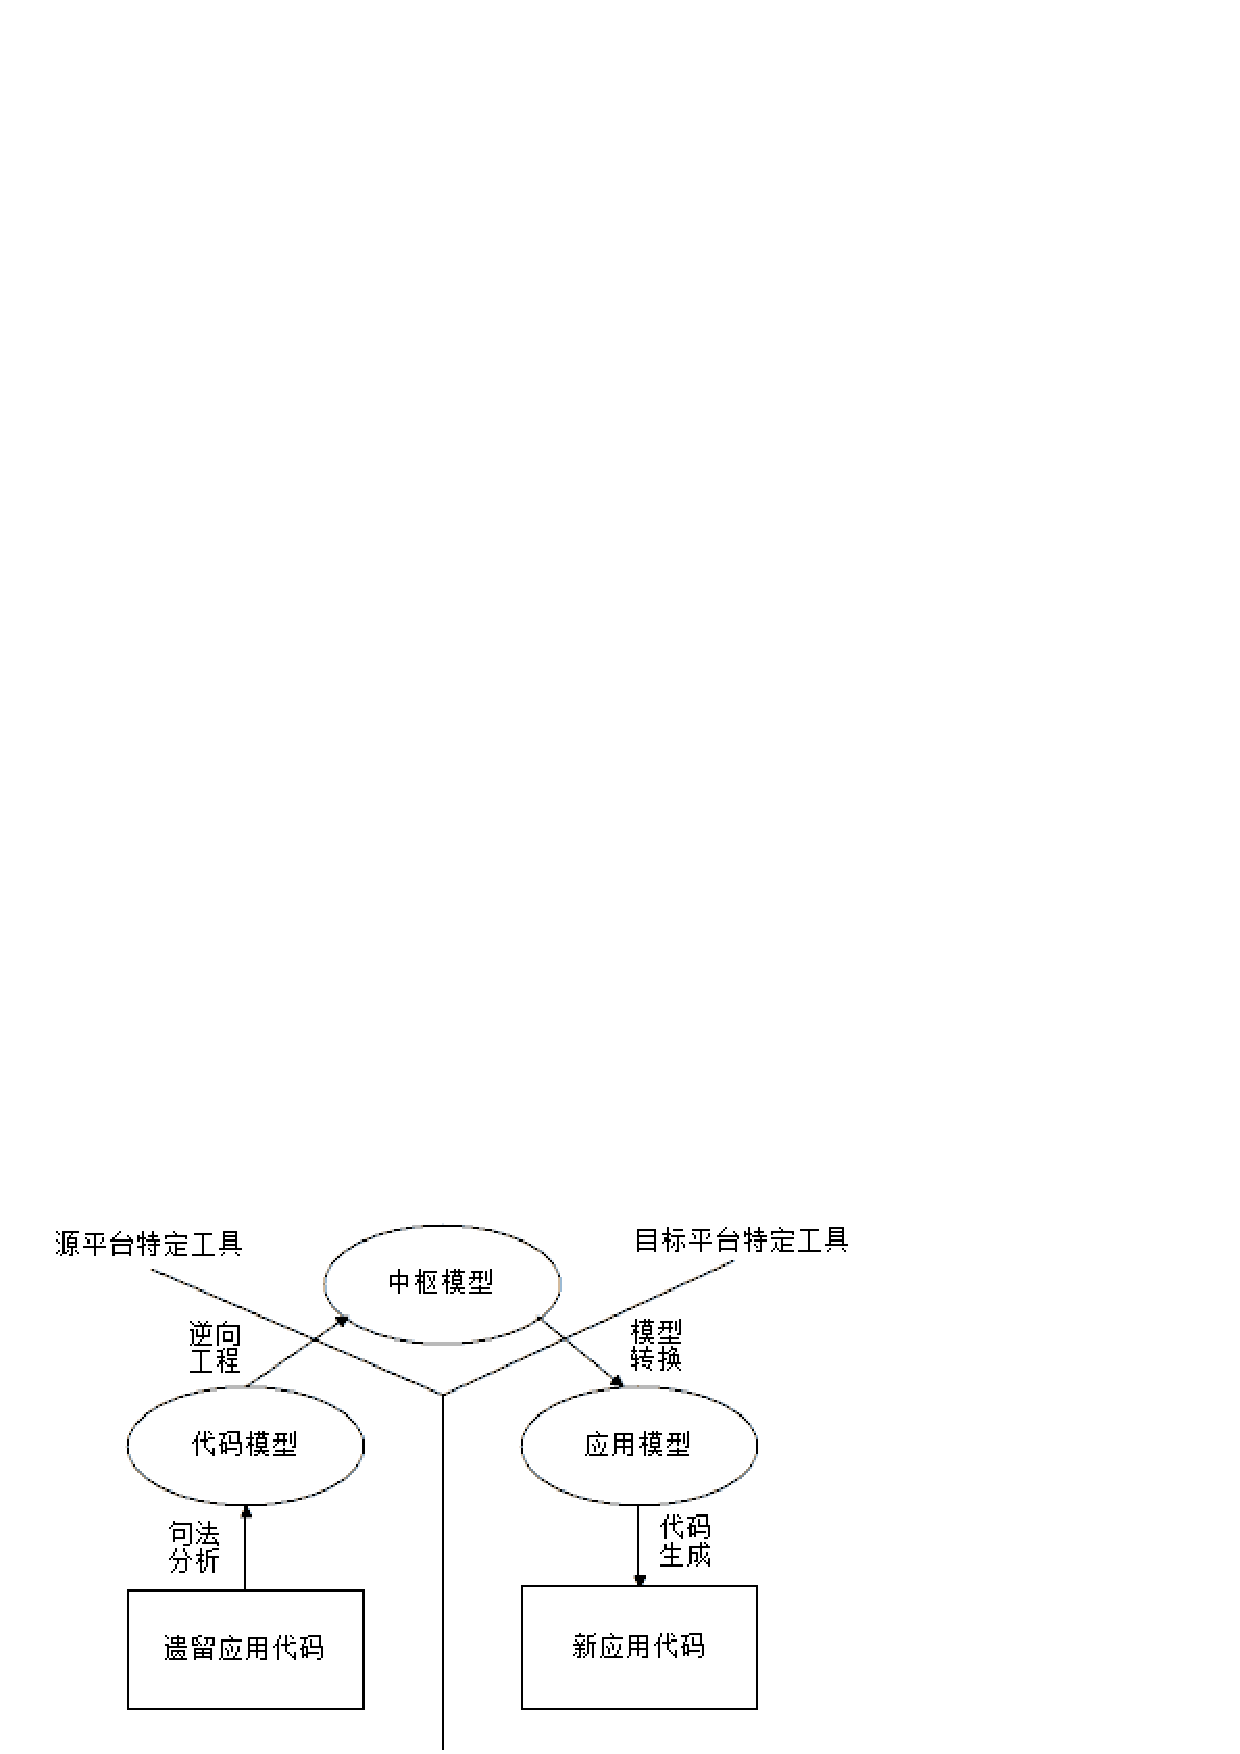
\includegraphics[width=200bp]{figure/pic/model-driving-software-porting.png}
    \caption{模型驱动工程的方法进行源代码移植}
    \label{model-driving-software-porting-sample}
\end{figure}

这一方法概述如下:首先对遗留应用的程序源代码本身进行分词和句法析构,生成应用代码模型。
在完整了解遗留应用的前提下,通过对代码模型进行逆向工程,生成一个通用的中枢模型。
这一中枢模型具有可重用的特性,并且获取了索要移植的软件的全部信息,如:
静态结构,图形化用户界面,工作流(应用导航),方法和算法等。
接下来向目标环境进行模型翻译,转换为对应目标平台上的应用模型。
最后通过使用之前得到的应用模型进行代码生成操作得到目标环境下对应的应用。

段成戈\upcite{段成戈2008基于重构偏序规划的软件移植方法研究}先生提出了一个思路。利用偏序规划的方法,来对软件本身的结构进行重构。以此来简化软件移植的流程。
该方法基于软件的结构变动信息,构建初始状态库和目标库;
对目标库建立重构的操作集;然后基于重构偏序规划算法,生成操作序列;最后按照偏序规划算法中得到的操作序列,完成软件的迁移工作。

真对具体软件或者项目移植的解决方法的研究可根据源和
目标环境分成几个类别\upcite{torchiano2008software}。
包括但不限于操作系统 (operation system) 移植、数据库 (database) 移植、编程语言 (program language) 移植、体系结构 (system architecture) 移植和用户界面 (user interface) 移植。
C++到JavaScript属于编程语言移植。而从桌面平台到web平台则同时属于操作系统移植 (web可抽象成一个与操作系统无关而只与浏览器有关的平台)、
编程语言移植、体系结构移植 (浏览器只支持JavaScript) 和用户界面移植 (原生的位图/矢量界面到web的DOM系统)。
皇甫俊彦\upcite{皇甫俊彦2011大型金融信息系统从}进行了从C\#到Java移植的研究,
提出了大型金融信息系统的源代码移植方案。其方法是分类方法,把软件的源代码,分成几个部分,
比如XML界面文件,
数据库文件,逻辑代码等部分,然后针对不同部分的内容展开针对性的移植工作。
宋雨明\upcite{宋雨明2013iphone}进行了iOS平台到Android平台的软件移植工作的研究,
通过使用一系列的现有自动化工具,对逻辑代码、界面文件和资源文件进行针对性转换。

\subsection{传统软件向web移植的相关进展}

国内的开发者对于跨平台技术一直很热衷,
但是国内开发者研究的主题往往以 javascript 向安卓、ios 和桌面平台移植为主,
比如白鹭 egert 引擎和 cocos2d-js 引擎。
但鲜有对 C++向 javascript 的移植。
根据调研,仅有北京触控科技一家公司在产品 cocos2dx 2.x 的版本中,
使用了 emscripten 编译器将 C++ 代码编写的的游戏编译成 html5 版本;
在 cocos2dx 3.x 的版本中,将该功能移除。
推出了更适合 html5 开发者的 cocos2d-js。

国外企业和学者对于 C/S 软件向 B/S 移植则一直存在很大兴趣。

在互联网刚刚兴起时:

Microsoft 在传统软件移植 web 方面是研究比较早的。最出名的就是
Microsoft IE ActiveX 技术,该技术可以使用大量 win32 api,对于 windows 软
件移植代码量改动最小,几乎没有性能损失。但是需要安装插件,没认证过的插
件会被大多数安全软件拦截,并且只支持 windows 系统,不能应用于移动 web。
而且有很多安全问题。

Sun 公司和其后继者 Oracle 一直在持续改进 Java JNI \upcite{gordon1998essential} 技术。
该技术可以支持多种平台,浏览器兼容性好。但是操作系统跨平台需要额外工作,为每个平台
编译一个 Native 版本,需要目标平台安装 Java 且开启浏览器支持。

Adobe 公司为了方便传统软件向 flash 移植,开发了 flasCC 技术,该技术平
台兼容性比较好,而且 swf 文件可以脱离浏览器单独运行。但是目标机需要安装
flash player,移动设备现在大都不支持 flash player;而且渲染器需要重写,
3 维软件移植需要大量重写;价格高昂;编译过程非常缓慢。

Unity3D 公司也仿照 Adobe 公司的 flasCC 技术,推出了 unityWebPlayer 方
案,需要浏览器支持 PPAPI,但是只能移植 unity 平台开发的游戏,并且不支持
第三方插件,物理引擎和光照处理也不是很好。

在HTML5兴起之后

在 javascript 语言标准化制定完成(也即 ECMAscript 5.1 定稿)时,、,也恰逢
html5 技术兴起。

Google 为了方便 chrome web app 的开发,推出了 Google Native Client 技
术,简称 Google NaCl\upcite{metz2011google}。
NaCl 与 Native 性能差距不大,平台兼容性好。但是只支
持 chrome 浏览器 ,而且是 chrome web 应用,而不是网页。

Leaning Technologies 公司推出了 C++向 Javascript 编译器 Duetto,既可
以将 C++代码用于 web 应用的生成,也可以通过生成 node.js 脚本用于后端开发,
生成的 javascript 代码可以充分利用 javascript 的 JIT,性能较高。但是使用
LGPL 协议发布,商业不友好,开发完成程度不高,文档亦不够完善。

Mozilla 公司和 Epic 公司为了将 unreal engine runtime 移植到 web 上,开
发了基于 llvm+clang 的 C++ to Javascript 编译器, Emscripten\upcite{zakai2011emscripten},
可以使用 c++全部特性;依靠 asm.js \upcite{herman2013asm}解释器,将 javascript 直接解释为汇编代码运行,个别
测试效率超越 C++;支持 openGL ES 2.0 程序直接转变为 webGL \upcite{webgl20142}程序 。

Unity 公司在 2014 年开始 webGL 移植的实验。并使用 IL2CPP 技术和 Emscripten 编译器,将 C\#代码转换为 C++代码,再将 C++代码转换成 javascript 代码。使游戏移植到 webGL 上。并在 2015 年发布的 unity5.3 版本中,宣布 unity3D 已经完美支持 webGL 平台。


\subsection{本文主要研究内容}

本文主要研究内容是从C++到html5的传统软件移植的问题。
作者对现有的软件移植工作进行了总是,总结了嵌入的先进研究程序,包括:
软件移植的概率、分类、方法以及原则。同时移植一些具有代表性的传统软件到html5,
提取通用传统软件web移植的工作流。

主要研究内容如下:

\begin{enumerate}
    \item 对软件移植 (software migration) 理论以及传统软件web移植成果进行综述;
    \item 剖析emscripten的结构,说明emscripten的工作流程;
    \item 移植有代表性的几个传统软件到html5;
    \item 总结传统软件移植html5的方法。
\end{enumerate}

本文组织结构如下:

{\heiti 第 1 章 } 绪论。本章简要介绍传统软件向web移植的问题出现的时代背景,
当前软件移植理论的研究现状以及本论文的主要内容。

{\heiti 第 2 章 } 剖析emscripten的工具的作用,原理,以及简介webIDL技术。

{\heiti 第 3 章 } luaVM。移植luaVM到html5,并实现一个纯前端的lua交互式解释器。

{\heiti 第 4 章 } SQLite。移植SQLite到html5,并实现一个可以在JavaScript虚拟机中运行的运行的SQLite实例,
并支持完整的的CURD操作。

{\heiti 第 5 章 } box2d。移植box2d物理引擎到html5,并在canvas中使用。

{\heiti 第 6 章 } bullet physics。移植bullet物理引擎到html5,并在webgl中进行使用。
